% Esta sección describe el planteamiento del problema, objetivos y requisitos
% del sistema embebido IoT para monitoreo y control automático de cultivos de perejil.

% --- ESPACIADO GENERAL ---
\setstretch{1.2}
\setlength{\parskip}{6pt}

% --- ESPACIADO EN LISTAS ---
\setlist[itemize]{itemsep=6pt, topsep=6pt}
\setlist[enumerate]{itemsep=6pt, topsep=6pt}

% --- SANGRÍA ---
\setlength{\parindent}{15pt}

% ============================================================
\subsection{Descripción del problema}
% ============================================================

En los cultivos de hortalizas a pequeña escala, el riego y el control ambiental se realizan de forma manual. En el caso específico del perejil (\textit{Petroselinum crispum}), esta situación es crítica porque la especie es sensible tanto a la deficiencia hídrica como al exceso de temperatura, lo que afecta directamente su germinación —requiere humedad constante del sustrato entre 60 y 80\,\%— y su desarrollo vegetativo —temperatura óptima entre 15 y 25\,°C—.

El riego manual genera ineficiencias como uso excesivo o insuficiente del agua, variabilidad en la humedad del sustrato, estrés hídrico, exposición térmica no controlada y baja capacidad de seguimiento técnico del proceso. La ausencia de un mecanismo de protección solar automático agrava el problema durante las horas de alta irradiación.

El Grupo~G5 diseñará e implementará un prototipo portable de semillero con geometría triangular equiláteral, base de 40\,cm y perímetro máximo de 160\,cm. El sistema contará con los siguientes componentes principales:

\begin{itemize}
    \item Tarjeta de desarrollo \textbf{ESP32-WROOM}.

    \item Sensor \textbf{DHT11} para medición de temperatura y humedad relativa del aire.

    \item Sensor \textbf{YL-100} para medición de humedad volumétrica del sustrato.

    \item \textbf{Sistema de riego por goteo}: bomba sumergible de 5\,V con filtro de malla y tres goteros ajustables distribuidos sobre el sustrato.

    \item \textbf{Techo móvil} accionado por un servo-motor SG90: se cierra automáticamente cuando la temperatura supera el umbral definido (\texttt{TEMP\_MAX}), protegiendo el cultivo de la irradiación solar directa, y se abre cuando la temperatura desciende por debajo de \texttt{TEMP\_MAX\,-\,HYSTERESIS\_T}.

    \item Plataforma IoT \textbf{ThingSpeak} con publicación de datos vía protocolo \textbf{MQTT} (broker \texttt{mqtt3.thingspeak.com}).

    \item Semilla de \textbf{perejil} (\textit{Petroselinum crispum}), suministrada por la docente encargada del proyecto.
\end{itemize}

\noindent\textbf{Problema central:} El cultivo experimental de perejil carece de un sistema automático capaz de mantener condiciones óptimas de humedad del sustrato y temperatura ambiental, activar el riego por goteo de forma autónoma, controlar un techo móvil para protección solar y visualizar remotamente el estado del sistema en ThingSpeak, reduciendo la necesidad de intervención manual continua.

% ============================================================
\subsection{Objetivos}
% ============================================================

\subsubsection{Objetivo general}

Diseñar e implementar un sistema embebido IoT para el monitoreo remoto y control automático de variables asociadas al crecimiento de perejil en un prototipo triangular portable con techo móvil, integrando los sensores DHT11 y YL-100, actuadores de riego por goteo y servo-motor para el control del techo, comunicación inalámbrica Wi-Fi mediante ESP32-WROOM y visualización remota en ThingSpeak vía MQTT.

\subsubsection{Objetivos específicos}

\begin{enumerate}
    \item Definir los requisitos funcionales y no funcionales del sistema, considerando las variables medidas por el DHT11 y el YL-100, y los requerimientos agronómicos de germinación y crecimiento del perejil.

    \item Diseñar la arquitectura hardware/software y el diseño físico 3D del prototipo, justificando la selección de la tarjeta ESP32-WROOM, los sensores, los actuadores, el mecanismo de techo móvil y la plataforma ThingSpeak.

    \item Implementar el prototipo funcional sobre el contenedor triangular, incorporando lógica de control con histéresis para el riego y la apertura/cierre del techo, y comunicación remota vía MQTT hacia ThingSpeak.

    \item Validar el sistema mediante pruebas experimentales documentadas en bitácora técnica y repositorio GitHub con historial de commits organizado.
\end{enumerate}

\subsection{Requisitos funcionales}
% ============================================================

La Tabla~\ref{tab:rf_proyectofinal} presenta los requisitos funcionales identificados para el sistema, definidos mediante el código RF-XX.

\begin{table*}[tp]
\centering
\renewcommand{\arraystretch}{1.3}
\caption{Requisitos Funcionales del Sistema -- Grupo G5}
\label{tab:rf_proyectofinal}
\begin{tabularx}{\textwidth}{|c|X|c|c|}
\hline
\textbf{ID} & \textbf{Descripción} & \textbf{Prioridad} & \textbf{Fuente} \\
\hline
RF-01 & Leer temperatura ambiente con DHT11, mínimo 1 lectura cada 5 s. & Alta & Enunciado XI \\
\hline
RF-02 & Leer humedad relativa del aire con DHT11, misma frecuencia que RF-01. & Alta & Enunciado XI \\
\hline
RF-03 & Leer humedad del sustrato con YL-100 (salida analógica al ADC), mínimo 1 lectura cada 10 s. & Alta & Enunciado XI \\
\hline
RF-04 & Activar la bomba de riego por goteo cuando humedad\_sustrato < HUMIDITY\_MIN. & Alta & Enunciado XIII-A \\
\hline
RF-05 & Desactivar la bomba de riego cuando humedad\_sustrato > HUMIDITY\_MIN + HYSTERESIS. & Alta & Enunciado XIII-A \\
\hline
RF-06 & Cerrar el techo móvil (servo a 90°) cuando temperatura > TEMP\_MAX, para proteger el cultivo del calor y la irradiación solar directa. & Alta & Enunciado XIII-B / Acta 1 \\
\hline
RF-07 & Abrir el techo móvil (servo a 0°) cuando temperatura < TEMP\_MAX $-$ HYSTERESIS\_T. & Alta & Enunciado XIII-B \\
\hline
RF-08 & Publicar en ThingSpeak vía MQTT las 5 variables del sistema con intervalo máx. de 15 s. & Alta & Enunciado XIV / ThingSpeak API \\
\hline
RF-09 & Cada publicación IoT debe serializar los datos en formato de campo ThingSpeak (field1\ldots field5) compatible con mqtt3.thingspeak.com. & Alta & ThingSpeak Docs \\
\hline
RF-10 & Implementar temporización no bloqueante con millis() --- sin uso de delay() en el bucle principal. & Alta & Enunciado XVI \\
\hline
RF-11 & Incluir filtro mecánico del agua (malla) antes de la línea de riego por goteo. & Alta & Acta 1 núm. 8 \\
\hline
RF-12 & Operar sobre contenedor triangular: base 40 cm, perímetro máx. 160 cm, altura sustrato mín. 10 cm. & Alta & Acta 1 núm. 4, 6 \\
\hline
RF-13 & Organizar firmware en módulos: readSensors(), controlIrrigation(), controlRoof(), publishThingSpeak(), updateActuators(). & Media & Enunciado XVI \\
\hline
\end{tabularx}
\end{table*}

% ============================================================
\subsection{Requisitos no funcionales}
% ============================================================

La Tabla~\ref{tab:rnf_proyectofinal} presenta los requisitos no funcionales identificados para el sistema, definidos mediante el código RNF-XX.

\begin{table*}[tp]
\centering
\renewcommand{\arraystretch}{1.3}
\caption{Requisitos No Funcionales del Sistema -- Grupo G5}
\label{tab:rnf_proyectofinal}
\begin{tabularx}{\textwidth}{|c|X|c|c|}
\hline
\textbf{ID} & \textbf{Descripción} & \textbf{Categoría} & \textbf{Fuente} \\
\hline
RNF-01 & Firmware en VS Code con PlatformIO. Prohibido .ino y Arduino IDE. & Restricción & Enunciado X \\
\hline
RNF-02 & Código en GitHub con historial de commits organizado que evidencie avance progresivo. & Trazabilidad & Enunciado X \\
\hline
RNF-03 & Operación continua mínimo 30 min sin fallos de sensor, actuador ni desconexión IoT. & Disponibilidad & Enunciado XXI \\
\hline
RNF-04 & Prototipo portable, peso estimado menor a 5 kg en operación completa. & Portabilidad & Acta 1 núm. 3 \\
\hline
RNF-05 & Latencia máxima de 15 s desde adquisición hasta actualización de canal en ThingSpeak (restricción free-tier). & Rendimiento & ThingSpeak API \\
\hline
RNF-06 & Contenedor sin fugas durante pruebas de riego; con sistema de drenaje. & Fiabilidad & Acta 1 núm. 6 \\
\hline
RNF-07 & ESP32 y conexiones protegidas de salpicaduras durante operación del riego. & Seg. eléctrica & Diseño propio \\
\hline
RNF-08 & Alimentación 5 V DC USB o power bank para demostración en laboratorio. & Energía & Diseño propio \\
\hline
RNF-09 & El techo móvil debe abrir y cerrar en menos de 3 s desde la activación del servo. & Rendimiento & Diseño propio \\
\hline
RNF-10 & Documentación de evidencias en bitácora técnica con fecha y responsables. & Documentación & Enunciado XVII-D \\
\hline
\end{tabularx}
\end{table*}

\subsection{Diagrama General del Sistema}
% ============================================================

\subsubsection{Arquitectura de Capas}
El sistema se organiza en cuatro capas funcionales. El flujo de datos es bidireccional entre el ESP32 y ThingSpeak, y se organiza como se muestra en la Figura \ref{fig:diagrama-capas}.

\begin{figure}[tp]
    \centering
    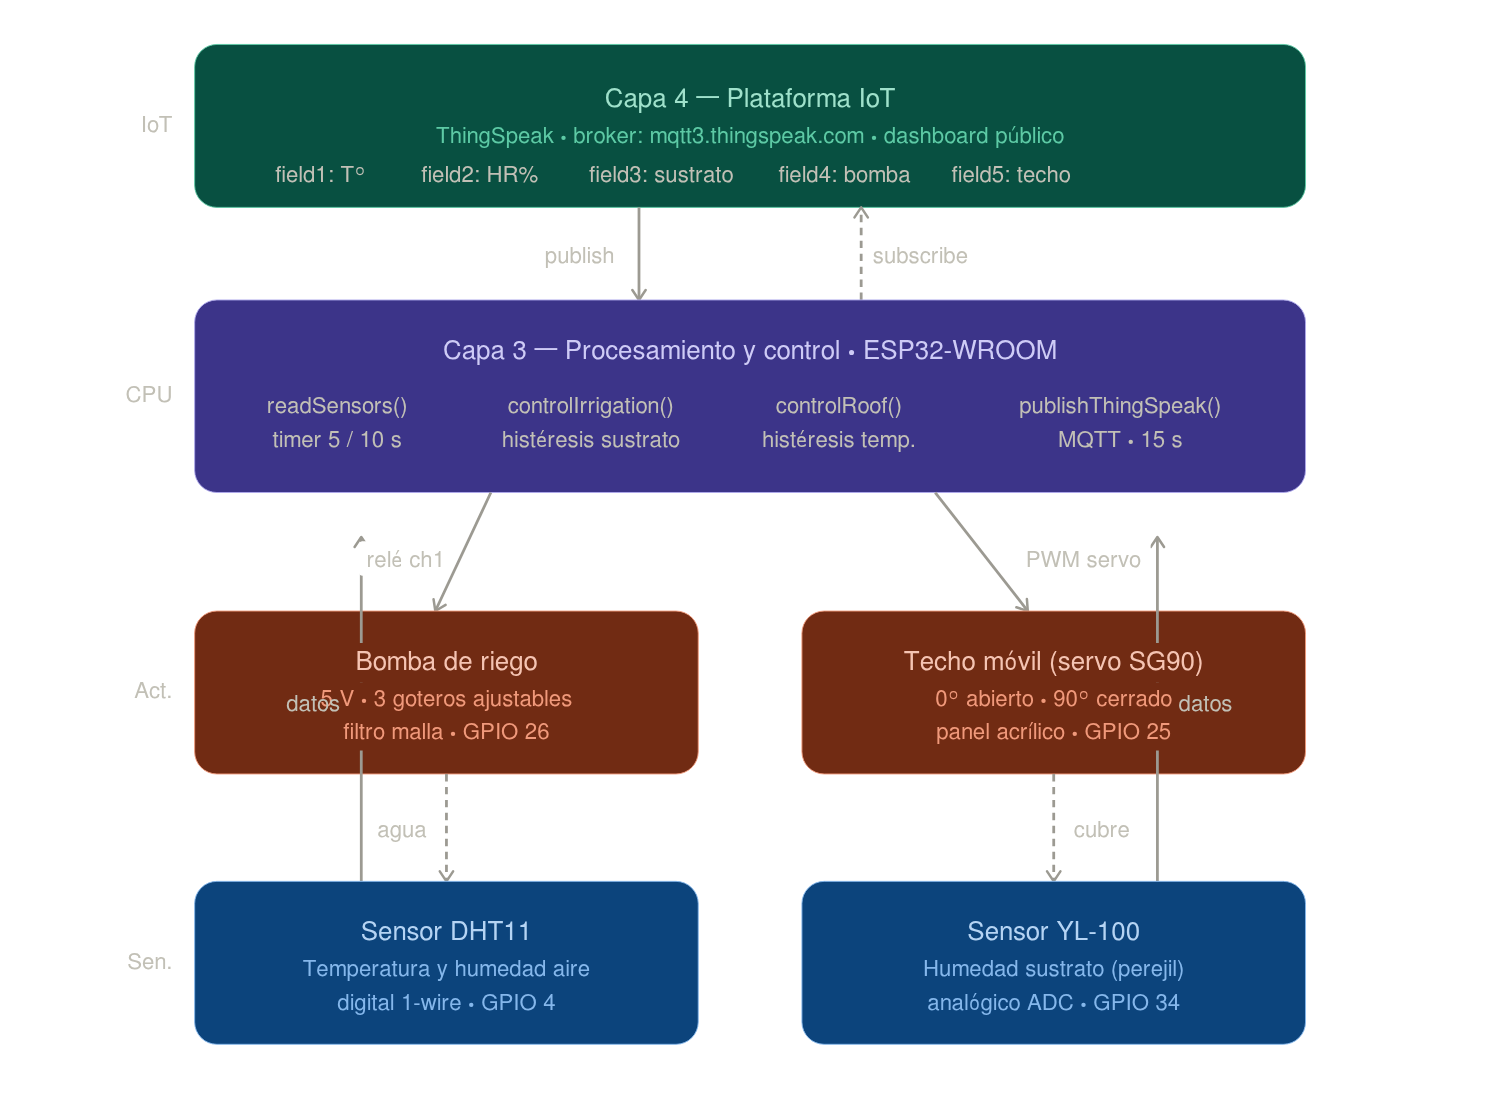
\includegraphics[width=\columnwidth]{images/diagrama-capas}
    \caption{Arquitectura de capas del sistema}
    \label{fig:diagrama-capas}
\end{figure}

\subsubsection{Variables del Sistema}

Las variables mínimas del sistema se resumen en la Tabla~\ref{tab:variables_sistema}, con su tipo, sensor/actuador asociado, rango de valores y uso específico dentro del sistema.

\begin{table*}[tp]
\centering
\renewcommand{\arraystretch}{1.3}
\caption{Variables Mínimas del Sistema}
\label{tab:variables_sistema}
\begin{tabularx}{\textwidth}{|c|c|c|c|X|}
\hline
\textbf{Variable} & \textbf{Tipo} & \textbf{Sensor/Actuador} & \textbf{Rango} & \textbf{Uso} \\
\hline
temperatura & Entrada & DHT11 & 0--50 °C & Control techo / monitoreo \\
\hline
humedad\_aire & Entrada & DHT11 & 20--90 \%HR & Monitoreo ambiental \\
\hline
humedad\_sustrato & Entrada & YL-100 (ADC) & 0--4095 (12-bit) & Activación riego \\
\hline
estado\_bomba & Salida & Relé + bomba & ON / OFF & Control irrigación \\
\hline
estado\_techo & Salida & Servo-motor & ABIERTO / CERRADO & Protección térmica/solar \\
\hline
\end{tabularx}
\end{table*}

\subsubsection{Flujo de Control del Firmware}

El firmware opera con un bucle principal no bloqueante (millis()). En cada iteración se evalúan tres temporizadores independientes:

\begin{itemize}
    \item \textbf{Timer sensores (5/10 s):} llama a \texttt{readSensors()} --- lee DHT11 y YL-100, valida rangos.
    \item \textbf{Timer control:} llama a \texttt{controlIrrigation()} con histéresis sobre \texttt{humedad\_sustrato}; luego \texttt{controlRoof()} con histéresis sobre temperatura; luego \texttt{updateActuators()} (GPIO relé + PWM servo).
    \item \textbf{Timer IoT (15 s):} llama a \texttt{publishThingSpeak()} --- publica los 5 campos en el canal ThingSpeak vía MQTT.
\end{itemize}

\section{Diseño Físico 3D del Prototipo}

\subsection{Descripción General}

El prototipo es un semillero portable con base cuadrada y paredes de acrílico transparente, sostenido por una estructura de perfiles de aluminio extruido. La Figura~\ref{fig:vista-isometrica} muestra la vista isométrica del diseño en SolidWorks. El ensamble completo se compone de cuatro módulos: (1) contenedor cuadrado con sustrato y paredes transparentes para visualización de raíces, (2) sistema hidráulico de riego por goteo con tres ramales, (3) techo móvil triangular de acrílico accionado por servo-motor 
MG995, y (4) caja electrónica lateral con ESP32-WROOM, pantalla OLED y módulo relé.

\begin{figure}[tp]
    \centering
    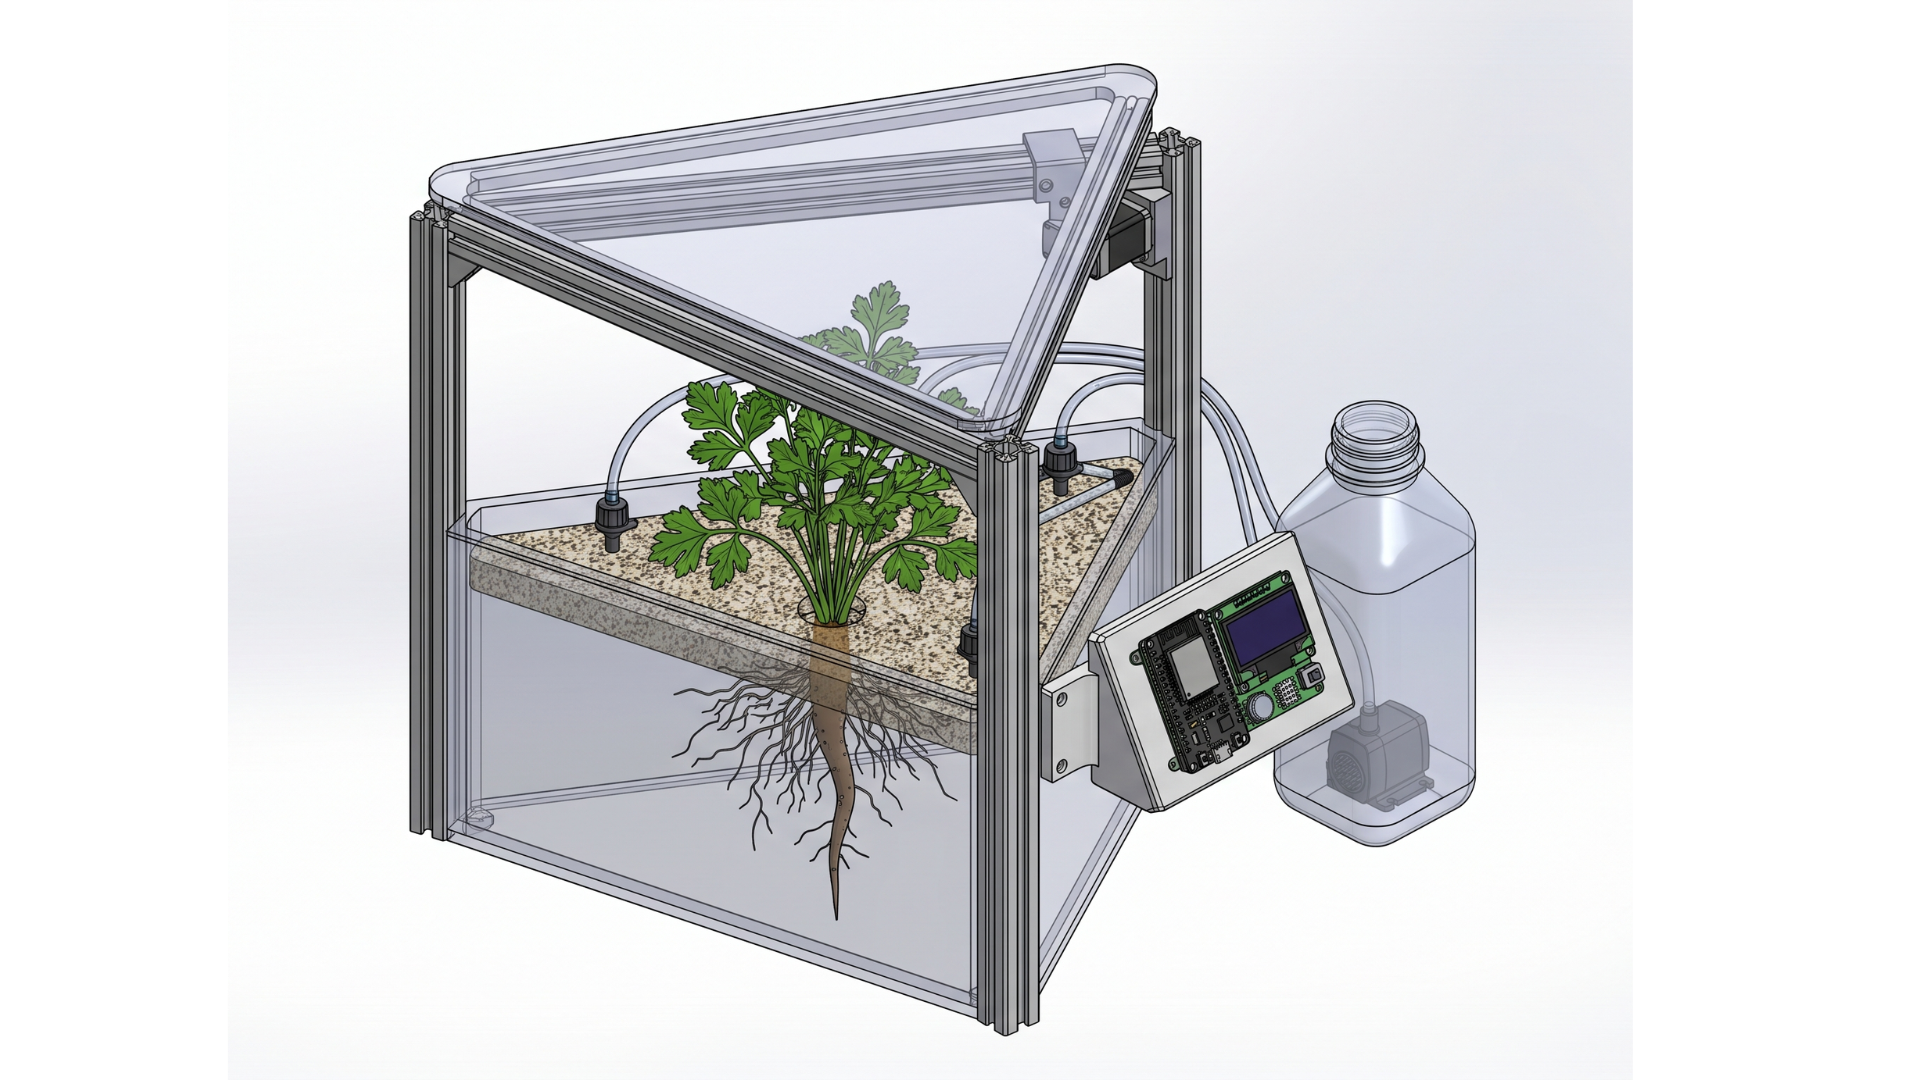
\includegraphics[width=\columnwidth]{images/vista-isometrica.png}
    \caption{Vista isométrica del prototipo: diseño en SolidWorks.}
    \label{fig:vista-isometrica}
\end{figure}

\subsection{Contenedor}

El contenedor tiene forma de prisma de base cuadrada con paredes de acrílico transparente de 3~mm, lo que permite la observación directa del sistema radicular del perejil. La estructura está reforzada con perfiles de aluminio extruido en los bordes. Sus dimensiones garantizan las restricciones del Acta~1, como se muestra en la Tabla~\ref{tab:dimensiones_contenedor}.

\begin{table*}[tp]
\centering
\renewcommand{\arraystretch}{1.3}
\caption{Dimensiones del Contenedor}
\label{tab:dimensiones_contenedor}
\begin{tabularx}{\textwidth}{|c|c|X|}
\hline
\textbf{Parámetro} & \textbf{Valor} & \textbf{Justificación} \\
\hline
Forma de la base & Cuadrado & Facilita la construcción y distribución uniforme de goteros \\
\hline
Lado de la base & $\sim$40 cm & Área suficiente para cultivo de perejil; cumple restricciones Acta~1 \\
\hline
Altura de la pared & 15 cm & Sustrato $\geq$ 10 cm (5 cm reserva drenaje) \\
\hline
Profundidad del sustrato & 10 cm & Permite inserción YL-100 a 5 cm; espacio para raíces \\
\hline
Profundidad de siembra & 1 cm & Estándar para semillas de perejil \\
\hline
Material paredes & Acrílico transparente 3 mm & Permite observación del sistema radicular \\
\hline
Estructura soporte & Perfil de aluminio extruido & Rigidez, bajo peso y ensamble modular \\
\hline
Sistema de drenaje & Orificios en la base & Evita exceso de agua en el sustrato \\
\hline
\end{tabularx}
\end{table*}

\subsection{Sistema Hidráulico de Riego por Goteo}

El sistema de riego consiste en una bomba sumergible de 5~V conectada a una tubería principal de silicona ($\varnothing$~4~mm) que se distribuye en tres ramales, cada uno con un gotero ajustable posicionado sobre el sustrato. Antes del ingreso del agua a la línea principal se instala un filtro de malla para proteger los goteros de obstrucciones. Los componentes se detallan en la Tabla~\ref{tab:componentes_hidraulicos}.

\begin{table*}[tp]
\centering
\renewcommand{\arraystretch}{1.3}
\caption{Componentes del Sistema Hidráulico}
\label{tab:componentes_hidraulicos}
\begin{tabularx}{\textwidth}{|l|c|X|}
\hline
\textbf{Componente} & \textbf{Cantidad} & \textbf{Especificación / Ubicación} \\
\hline
Bomba sumergible 5 V & 1 & Depósito lateral; caudal $\sim$120 L/h; control vía relé ch1 \\
\hline
Gotero ajustable & 3 & Distribuidos uniformemente en el triángulo, sobre el sustrato \\
\hline
Manguera silicona $\varnothing$ 4 mm & $\sim$60 cm & Recorre el perímetro interno del contenedor \\
\hline
Conectores T $\varnothing$ 4 mm & 3 & Derivaciones hacia cada gotero \\
\hline
Filtro de malla & 1 & Instalado a la salida de la bomba, antes de la línea principal \\
\hline
Tapón final & 1 & Cierre del extremo de la manguera para evitar fugas \\
\hline
Depósito de agua & 1 & Recipiente exterior al contenedor; capacidad $\sim$500 mL \\
\hline
\end{tabularx}
\end{table*}

\subsection{Estructura Soporte y Techo Móvil}

La estructura de soporte consiste en perfiles de aluminio extruido en los cuatro bordes verticales del contenedor. Sobre la parte superior se monta el mecanismo de techo móvil.

El techo móvil es un panel triangular de acrílico transparente, unido al marco superior por una bisagra metálica en uno de los lados del cuadrado. El servo-motor MG995 está fijado en la esquina opuesta a la bisagra y controla la apertura y el cierre del panel:

\begin{itemize}
    \item \textbf{Servo a 0°:} techo completamente abierto (máxima ventilación y luz).
    \item \textbf{Servo a 90°:} techo completamente cerrado (protección contra irradiación solar directa y exceso de temperatura).
    \item La transición tarda menos de 3~s (RNF-09).
\end{itemize}

Las especificaciones del techo móvil y el servo se presentan en la Tabla~\ref{tab:techo_servo}.

\begin{table*}[tp]
\centering
\renewcommand{\arraystretch}{1.3}
\caption{Especificaciones del Techo Móvil y Servo}
\label{tab:techo_servo}
\begin{tabularx}{\textwidth}{|c|c|X|}
\hline
\textbf{Parámetro} & \textbf{Valor} & \textbf{Observación} \\
\hline
Actuador & Servo MG995 & Torque 1.8 kg$\cdot$cm @ 5 V; control PWM 50 Hz \\
\hline
Pin de control & GPIO 25 (ESP32) & Señal PWM: pulso 1 ms (0°) --- 2 ms (90°) \\
\hline
Posición ABIERTO & 0° (servo) & Techo en posición horizontal, paralelo al suelo \\
\hline
Posición CERRADO & 90° (servo) & Panel cubre el cultivo completamente \\
\hline
Material del panel & Acrílico opaco 3 mm & Bloquea irradiación solar directa \\
\hline
Fijación bisagra & Lado A del triángulo (40 cm) & Bisagra metálica de piano, resistente a la humedad \\
\hline
Umbral cierre & Temperatura $>$ \texttt{TEMP\_MAX} (25°C) & Configurable en \texttt{config.h} \\
\hline
Umbral apertura & Temperatura $<$ \texttt{TEMP\_MAX} $-$ \texttt{HYSTERESIS\_T} (22°C) & Con histéresis de 3°C por defecto \\
\hline
\end{tabularx}
\end{table*}

\subsection{Caja Electrónica}

La electrónica del sistema se aloja en una caja de PVC o impresión 3D adosada lateralmente al contenedor triangular. La caja incluye:

\begin{itemize}
    \item Módulo ESP32-WROOM montado sobre protoboard o PCB perforada.
    \item Módulo relé de 1 canal para la bomba de riego.
    \item Conector para el servo MG995 (cable de 3 hilos: VCC, GND, PWM).
    \item Sensor DHT11 con orificio de ventilación en la caja (exposición al aire).
    \item Conector micro-USB para alimentación desde power bank.
    \item Tornillos de acceso para mantenimiento.
\end{itemize}

La distribución de pines del ESP32-WROOM se presenta en la Tabla~\ref{tab:pines_esp32}.

\begin{table*}[tp]
\centering
\renewcommand{\arraystretch}{1.3}
\caption{Distribución de Pines del ESP32-WROOM}
\label{tab:pines_esp32}
\begin{tabularx}{\textwidth}{|c|c|c|X|}
\hline
\textbf{Pin GPIO} & \textbf{Componente} & \textbf{Modo} & \textbf{Descripción} \\
\hline
GPIO 4 & DHT11 & Digital Input & Lectura de temperatura y humedad relativa del aire \\
\hline
GPIO 34 & YL-100 & ADC Input & Lectura analógica de humedad del sustrato (0--4095) \\
\hline
GPIO 26 & Relé bomba & Digital Output & Activación/desactivación de la bomba de riego (trigger LOW) \\
\hline
GPIO 25 & Servo SG90 & PWM Output & Control angular del techo móvil (0° abierto / 90° cerrado) \\
\hline
3.3 V & DHT11 / YL-100 & Power & Alimentación de sensores \\
\hline
5 V (Vin) & Servo SG90 / Relé & Power & Alimentación de actuadores \\
\hline
\end{tabularx}
\end{table*}

\section{Selección Justificada de la Tarjeta}

\subsection{Tarjeta Asignada: ESP32-WROOM}

Conforme al Acta 1, el Grupo~G5 utiliza la tarjeta ESP32-WROOM. La Tabla~\ref{tab:comparativa_tarjetas} compara las tres opciones disponibles en el proyecto.

\begin{table*}[tp]
\centering
\renewcommand{\arraystretch}{1.3}
\caption{Comparativa de Tarjetas de Desarrollo}
\label{tab:comparativa_tarjetas}
\begin{tabularx}{\textwidth}{|X|c|c|c|}
\hline
\textbf{Criterio} & \textbf{ESP32-WROOM} $\checkmark$ & \textbf{STM32 Nucleo} & \textbf{RPi Pico W} \\
\hline
Wi-Fi integrado & Sí (802.11 b/g/n) & No (módulo externo) & Sí (CYW43439) \\
\hline
Entradas ADC & 18 ch / 12 bit & Hasta 16 ch / 12 bit & 3 ch / 12 bit \\
\hline
Salidas PWM (servo) & 16 canales LEDC & Timers dedicados & 16 canales PIO \\
\hline
Soporte MQTT/ThingSpeak & PubSubClient + ESP32 & Complejo, no nativo & Básico (umqtt) \\
\hline
Procesador & Dual-core 240 MHz & Cortex-M4 180 MHz & Dual-core 133 MHz \\
\hline
PlatformIO / VS Code & Muy fácil & Fácil & Medio \\
\hline
Nivel lógico GPIO & 3.3 V & 3.3 V & 3.3 V \\
\hline
\end{tabularx}
\end{table*}

\subsection{Justificación}

\begin{enumerate}
    \item \textbf{Conectividad Wi-Fi nativa:} elimina hardware adicional para la comunicación MQTT con ThingSpeak, reduciendo costo y complejidad del diseño.
    \item \textbf{PWM para servo:} el módulo LEDC del ESP32 genera señales PWM de 50~Hz con resolución de 16 bits, ideal para el control preciso del servo SG90 del techo móvil.
    \item \textbf{Librerías maduras para ThingSpeak:} PubSubClient permite la conexión al broker \texttt{mqtt3.thingspeak.com}; ArduinoJson facilita el formateo de payloads. Ambas están disponibles en PlatformIO.
    \item \textbf{ADC de 12 bits:} la salida analógica del YL-100 se conecta directamente al GPIO~34 con rango 0--4095, sin circuito acondicionador adicional.
    \item \textbf{Dual-core 240~MHz:} permite gestionar concurrentemente el control del servo, el riego, la lectura de sensores y la publicación MQTT sin bloqueos.
\end{enumerate}

\section{Sensores y Actuadores}

\subsection{Sensores}

La Tabla~\ref{tab:sensores} presenta los sensores utilizados en el sistema.


\begin{table*}[tp]
\centering
\renewcommand{\arraystretch}{1.3}
\caption{Sensores del Sistema}
\label{tab:sensores}
\begin{tabularx}{\textwidth}{|c|c|X|}
\hline
\textbf{Sensor} & \textbf{Interfaz / Rango} & \textbf{Variable medida y justificación} \\
\hline
DHT11 & Digital 1-wire / 0--50°C, 20--90\%HR & Temperatura y humedad del aire. Bajo costo, librería Adafruit en PlatformIO, compatible 3.3~V. \\
\hline
YL-100 & Analógica ADC / 0--4095 (12-bit) & Humedad del sustrato. Salida directa al ADC del ESP32, alimentación 3.3~V, disponible en laboratorio. \\
\hline
\end{tabularx}
\end{table*}

\noindent\textbf{Nota de calibración YL-100:} se tomarán lecturas ADC en sustrato seco (valor máximo $\approx$60\,\% escala) y sustrato saturado (valor mínimo) durante el Entregable~2 para definir \texttt{HUMIDITY\_MIN} y \texttt{HUMIDITY\_MAX}. El perejil requiere humedad del sustrato entre 60 y 80\,\% para germinación.

\subsection{Actuadores}

La Tabla~\ref{tab:actuadores} presenta los actuadores utilizados en el sistema.

% Table_Actuadores.tex
\begin{table*}[tp]
\centering
\renewcommand{\arraystretch}{1.3}
\caption{Actuadores del Sistema}
\label{tab:actuadores}
\begin{tabularx}{\textwidth}{|c|c|X|}
\hline
\textbf{Componente} & \textbf{Control / Alimentación} & \textbf{Función y justificación} \\
\hline
Bomba sumergible 5~V & Relé ch1 + GPIO~26 / 5~V DC $\sim$300~mA & Riego por goteo (3 goteros). Control on/off mediante relé. \\
\hline
Servo-motor SG90 & PWM GPIO~25 (50~Hz) / 5~V DC $\sim$250~mA & Apertura/cierre del techo móvil. Torque 1.8~kg$\cdot$cm, control angular preciso. \\
\hline
Módulo relé 1 canal & GPIO 3.3~V (trigger LOW) / 5~V bobina & Aislamiento ESP32--bomba. Optoacoplador protege el ESP32. \\
\hline
\end{tabularx}
\end{table*}

\section{Plataforma IoT --- ThingSpeak con MQTT}

\subsection{Descripción de ThingSpeak}

ThingSpeak es una plataforma IoT en la nube de MathWorks que permite recibir, almacenar y visualizar datos de sensores mediante canales con hasta 8 campos. Se integra nativamente con MATLAB para análisis y cuenta con soporte para el protocolo MQTT a través del broker \texttt{mqtt3.thingspeak.com} (puerto 1883 o 8883 TLS).

Se utiliza la cuenta free-tier de ThingSpeak, que impone una tasa mínima de actualización de 15 segundos por canal, por lo que el timer IoT del firmware se configura con un intervalo de 15~s (RF-08, RNF-05).

\subsection{Configuración del Canal ThingSpeak}

La Tabla~\ref{tab:thingspeak_campos} presenta la configuración del canal ThingSpeak del Grupo~G5.

\begin{table*}[tp]
\centering
\renewcommand{\arraystretch}{1.3}
\caption{Configuración del Canal ThingSpeak --- Grupo G5}
\label{tab:thingspeak_campos}
\begin{tabularx}{\textwidth}{|c|c|X|}
\hline
\textbf{Campo (Field)} & \textbf{Variable publicada} & \textbf{Descripción} \\
\hline
field1 & \texttt{temperatura} & Temperatura ambiente en °C (float, 1 decimal) \\
\hline
field2 & \texttt{humedad\_aire} & Humedad relativa del aire en \% (float, 0 decimales) \\
\hline
field3 & \texttt{humedad\_sustrato} & Humedad del sustrato en \% escalado (float, 0--100) \\
\hline
field4 & \texttt{estado\_bomba} & Estado de la bomba de riego: 1 = ON, 0 = OFF (int) \\
\hline
field5 & \texttt{estado\_techo} & Estado del techo: 1 = CERRADO, 0 = ABIERTO (int) \\
\hline
\end{tabularx}
\end{table*}

\subsection{Configuración MQTT}

Los parámetros de conexión MQTT se presentan en la Tabla~\ref{tab:mqtt_params}.

\begin{table*}[tp]
\centering
\renewcommand{\arraystretch}{1.3}
\caption{Parámetros de Conexión MQTT --- ThingSpeak}
\label{tab:mqtt_params}
\begin{tabularx}{\textwidth}{|c|X|}
\hline
\textbf{Parámetro} & \textbf{Valor} \\
\hline
Broker & \texttt{mqtt3.thingspeak.com} \\
\hline
Puerto & 1883 (TCP sin TLS) \\
\hline
Client ID & \texttt{<ThingSpeakClientID>} (generado en cuenta ThingSpeak) \\
\hline
Usuario & \texttt{<ThingSpeakUsername>} \\
\hline
Contraseña & \texttt{<API\_KEY\_Write\_del\_canal>} \\
\hline
Tópico de publicación & \texttt{channels/<channel\_id>/publish} \\
\hline
Formato del payload & \texttt{field1=28.5\&field2=71\&field3=65\&field4=0\&field5=1} \\
\hline
Intervalo mínimo & 15 segundos (restricción free-tier ThingSpeak) \\
\hline
Librería firmware & PubSubClient (Arduino/ESP32) \\
\hline
\end{tabularx}
\end{table*}

\subsection{Visualización en ThingSpeak}

Cada campo publicado se visualiza automáticamente en el dashboard del canal como gráfica de línea temporal. Se configurarán los siguientes widgets:

\begin{itemize}
    \item \textbf{Field~1 (temperatura):} gráfica de línea con banda de alerta a \texttt{TEMP\_MAX} = 25~°C.
    \item \textbf{Field~2 (humedad aire):} gráfica de línea.
    \item \textbf{Field~3 (humedad sustrato):} gráfica de línea con banda inferior a \texttt{HUMIDITY\_MIN} = 60~\%.
    \item \textbf{Field~4 (bomba riego):} indicador numérico ON/OFF.
    \item \textbf{Field~5 (estado techo):} indicador numérico ABIERTO/CERRADO.
\end{itemize}

\section{Partición Hardware/Software}

La Tabla~\ref{tab:funciones_hardware} asigna las funciones al hardware y la Tabla~\ref{tab:funciones_firmware} al firmware.

\begin{table*}[tp]
\centering
\renewcommand{\arraystretch}{1.3}
\caption{Funciones Asignadas al Hardware}
\label{tab:funciones_hardware}
\begin{tabularx}{\textwidth}{|X|X|}
\hline
\textbf{Función Hardware} & \textbf{Componente Responsable} \\
\hline
Medición de temperatura y humedad del aire & Sensor DHT11 \\
\hline
Medición de humedad del sustrato & Sensor YL-100 + ADC del ESP32 \\
\hline
Activación física de la bomba de riego & Módulo relé canal 1 + bomba sumergible 5 V \\
\hline
Activación física del actuador térmico & Módulo relé canal 2 + ventilador/atomizador \\
\hline
Aislamiento eléctrico de cargas & Módulo relé 2 canales con optoacoplador \\
\hline
Alimentación del sistema & Fuente 5 V DC USB / power bank \\
\hline
Filtrado mecánico del agua & Filtro de malla antes de la línea de goteo \\
\hline
Distribución del agua a los 3 goteros & Manguera + conectores T + 3 goteros ajustables \\
\hline
Contenedor del sustrato y semillas & Contenedor triangular (base 40 cm, altura mín. 10 cm) \\
\hline
\end{tabularx}
\end{table*}
\begin{table*}[tp]
\centering
\renewcommand{\arraystretch}{1.3}
\caption{Funciones Asignadas al Firmware (Software)}
\label{tab:funciones_firmware}
\begin{tabularx}{\textwidth}{|X|X|}
\hline
\textbf{Función Software} & \textbf{Módulo Firmware} \\
\hline
Lectura periódica de temperatura y humedad (DHT11) & readSensors() --- timer 5 s \\
\hline
Lectura periódica de humedad del sustrato (YL-100) & readSensors() --- timer 10 s \\
\hline
Validación de lecturas (rango válido, NaN, error) & readSensors() --- validación inline \\
\hline
Lógica de control de riego con histéresis & controlIrrigation() \\
\hline
Lógica de control térmico con histéresis & controlTemperature() \\
\hline
Actualización del estado de actuadores (GPIO) & updateActuators() \\
\hline
Serialización de datos en JSON & publishIoTData() --- ArduinoJson \\
\hline
Publicación de telemetría en MQTT / Firebase & publishIoTData() --- PubSubClient \\
\hline
Conexión Wi-Fi y reconexión automática & setup() + loop() --- WiFi.begin() \\
\hline
Temporización no bloqueante (sin delay()) & millis() + lastTime\_X \\
\hline
Constantes de umbrales y pines & config.h --- HUMIDITY\_MIN, TEMP\_MAX, \ldots \\
\hline
\end{tabularx}
\end{table*}